\documentclass[a4paper]{article}
\usepackage{amsfonts}
\usepackage{amsmath}
\usepackage{amssymb}
\usepackage{graphicx}     

\begin{document}
  
\noindent \large Auteur: Eryk Borczuch \\
\noindent \large Studierichting: Informatica\\
\noindent \large Oefeningenreeks 5F nr.1.9\\

\medskip

\normalsize

$r = 4+3 \cos \theta $ (limaçon)\\

$S = \dfrac{1}{2} \displaystyle \int_0^{2\pi} (4+3\cos \theta)^2 d\theta$\\

$= \dfrac{1}{2} \displaystyle \int_0^{2\pi} (16 +24 \cos \theta + 9 \cos^2 \theta) d \theta$\\

$= 16 \pi +12 [\sin \theta]_0 ^{2\pi} + \dfrac{9}{2} \displaystyle \int_0^{2\pi} \dfrac{1+ \cos (2 \theta)}{2} d \theta$\\

$\displaystyle = 16 \pi + \dfrac{9}{4} \int_0^{2\pi} d\theta + \dfrac{9}{4} \int_0^{2\pi}\cos(2\theta) d\theta$\\

$= 16\pi + \dfrac{9}{4}\pi + \dfrac{9}{8}[\sin(2\theta)]_0^{2\pi}$\\

$= 16\pi + \dfrac{9}{2}\pi$\\

$= \dfrac{41}{2}\pi$



\begin{figure}[htbp]
    \centering
    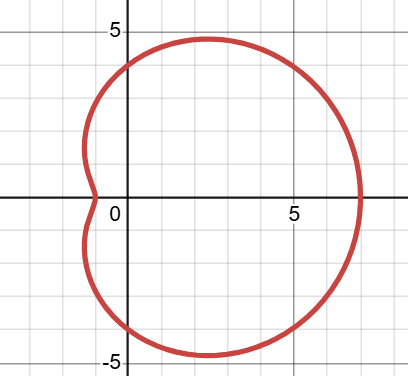
\includegraphics[width=0.7\linewidth]{5F-1.9-eryk.borczuch.INF.png}
\end{figure}


\begin{thebibliography}{999}
%\bibitem{a} Referentie
\end{thebibliography}
\end{document} 
